\chapter{Thesis project: Implementing a MLOps/GitOps workflow}\label{ch:thesis-project:-a-standard-mlops-ci/cd-workflow}
\chaptermark{Thesis : MLOps/GitOps WorkFlow}
\section{Introduction}\label{sec:introduction}
Building upon our state-of-the-art review of MLOps practices, this chapter introduces our practical implementation of a MLOps/GitOps workflow.
The proposed workflow is designed with versatility in mind—capable of enhancing existing projects at various maturity levels or providing a robust foundation for new initiatives seeking accelerated production deployment.

Rather than developing yet another platform, our approach integrates established tools and workflows identified in the literature into a cohesive system tailored to address modern machine learning development challenges.
A distinguishing feature of our implementation is the incorporation of GitOps principles into the MLOps workflow, creating a synergistic relationship between these complementary methodologies.

At the core of our design is the GitOps philosophy, which establishes Git repositories as the single source of truth for code, configurations, and infrastructure.
We leverage GitHub repositories as the central foundation, with GitHub Actions orchestrating our DevOps workflows.
This integration extends further through tools such as ArgoCD, GitSync, and custom scripts that trigger our DataOps and MLOps pipelines. % in a synchronized manner.

Our infrastructure is deployable across one or multiple Kubernetes clusters, depending on specific project requirements.
This architecture decouples the workflow definition from hardware considerations, offering significant flexibility.
The Kubernetes implementation supports dedicated nodes with specialized resources (high CPU, memory, GPU) for compute-intensive machine learning or data processing operations.
Furthermore, this approach accommodates diverse deployment scenarios:

\begin{itemize}
\item Cloud-based Kubernetes clusters
\item On-premises infrastructure
\item Single-node Kubernetes configurations running on development laptops (within hardware constraints)
\end{itemize}

The seamless integration of DevOps, DataOps, and MLOps pipelines culminates in a comprehensive MLOps workflow that is portable across any Kubernetes environment.
This integration addresses the full machine learning lifecycle from development to deployment while maintaining consistent practices. % throughout.

Our implementation was specifically developed to support our promoter's ongoing LSFB (Langue des Signes de Belgique Francophone) project, which is already operational in a production environment.
The practical application of our workflow to an existing, real-world machine learning system provided valuable insights into the challenges of MLOps adoption beyond theoretical constructs.
By enhancing the established LSFB project infrastructure, we could demonstrate the adaptability and incremental benefits of our approach while supporting continued model development and improvement for this important initiative.

In the following sections, we detail our use cases and the specific tools selected to implement our workflow and explain how they interconnect to create a modular system that can adapt as projects evolve in complexity and maturity.
Notably, our tool selection was significantly influenced by the existing LSFB project infrastructure.
The current production system consists of a Python-based model deployed as a Docker image that exposes an API consumed by a web frontend.
The project already utilizes GitHub for code management and Airflow for certain pipeline operations, which represents partial implementation of practices identified in our literature review.
These existing elements served as foundational components that our comprehensive workflow needed to accommodate and enhance rather than replace, demonstrating the practical flexibility of our approach.

\section{Use Case Definitions}\label{sec:use-case-definitions}
Before proceeding further, we formally outline the use cases this project aims to address.
We will describe our use case diagram displayed in figure~\ref{fig:usecases}.

\begin{figure}[!htbp]
    \centering
    \caption{Example of a MLOps pipeline define within Airflow}
    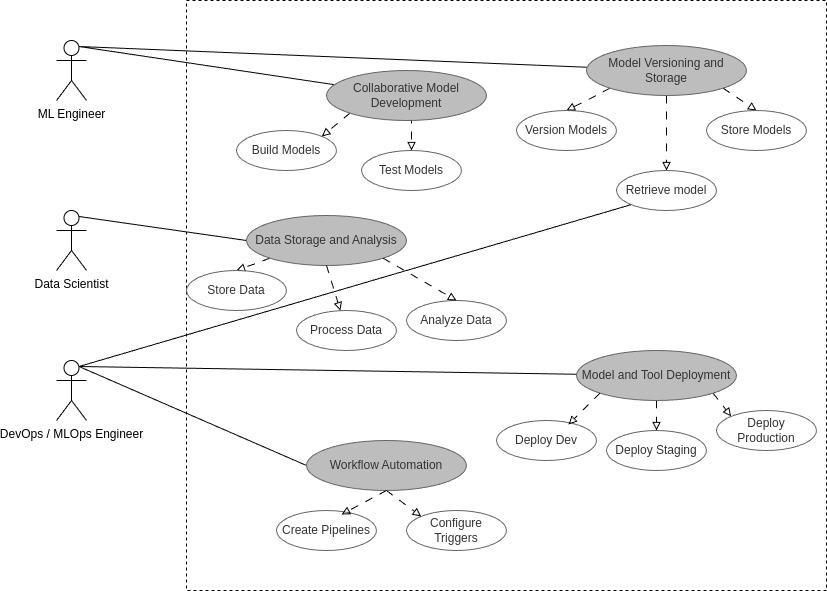
\includegraphics[scale=0.5]{images/project/usecases}
    \label{fig:usecases}
\end{figure}

\subsection{Collaborative Model Development}\label{subsec:collaborative-model-development}
The platform must provide the necessary tools and infrastructure to enable development teams to collaboratively build,
test, and deploy models across segregated environments.

\subsection{Data Storage and Analysis}\label{subsec:data-storage-and-analysis}
A robust system for storing, processing, and analyzing data is required to support model training and evaluation.

\subsection{Model Versioning and Storage}\label{subsec:model-versioning-and-storage}
The solution must include a structured approach to versioning, storing, and retrieving trained models efficiently.

\subsection{Model and Tool Deployment}\label{subsec:model-and-tool-deployment}
The system must support seamless deployment of models and associated tooling across environments—from local development
setups to production—with minimal friction.

\subsection{Workflow Automation}\label{subsec:workflow-automation}
To enhance operational maturity, we prioritize automating repetitive tasks in the workflow.
This will be achieved through well-defined pipelines and triggers, informed by our state-of-the-art review.
\section{Tools Selection Rationale}\label{sec:tools2}
Having established the theoretical foundations and component descriptions in our state-of-the-art review, this section focuses specifically on our tool selection rationale.
While our workflow is designed to be fundamentally tool-agnostic, the following choices were made to address the specific requirements of our implementation context, particularly the existing LSFB project infrastructure.

\subsection{Python}\label{subsec:python}
The foundational programming language for our entire workflow implementation, selected primarily to maintain compatibility with the LSFB project's existing codebase and the broader machine learning ecosystem.
The project's current use of Keras for model development and our demonstration implementations using scikit-learn both benefit from Python's extensive machine learning library ecosystem and developer familiarity.
Notably, Python's pervasive role extends to our pipeline implementations, as both Airflow DAGs and Kubeflow pipelines are defined using Python, creating a consistent development environment across all workflow components.

\subsection{Git Repositories and CI/CD}\label{subsec:github}
We selected GitHub as our version control and CI/CD platform primarily due to its established presence in the LSFB project ecosystem.
This choice provides continuity with existing development practices while enabling us to leverage GitHub Actions for workflow automation without introducing additional integration complexity.
GitHub's robust API and extensive integration capabilities further support our goal of building an interconnected MLOps workflow.

\subsection{IAC, Containers and Registry}\label{subsec:dockerhub}
Docker was the natural containerization choice given the LSFB project's existing Docker-based model deployment.
DockerHub serves as our container registry and Helm chart repository, offering reliable accessibility and established integration paths with our other selected tools.
This approach maintains compatibility with the current production environment while enabling more sophisticated deployment patterns.

\subsection{Kubernetes}\label{subsec:kubernetes}
Kubernetes was selected as our orchestration platform for its exceptional flexibility and robust ecosystem.
Its ability to operate across various infrastructure environments (cloud, on-premises, development workstations) directly supports our portability requirements.
Furthermore, Kubernetes provides the foundation for advanced deployment strategies needed in ML systems and enables seamless integration with specialized tools like Kubeflow and Airflow.


\subsection{Airflow}\label{subsec:airflow}
We chose Airflow for DataOps orchestration to maintain compatibility with existing pipelines in the LSFB project.
This selection allows us to extend current functionality while providing a bridge to new MLOps capabilities.
Airflow's Python-based DAG definitions integrate naturally with our development workflow and allow data scientists to define complex pipelines using familiar syntax.
Airflow's ability to trigger Kubeflow pipelines creates a unified workflow that respects team boundaries and specialized tooling preferences while maintaining end-to-end process integrity.
Moreover, by leveraging Airflow's recent GitSync capabilities, we were able to successfully implement GitOps principles within our MLOps project.

\subsection{Kubeflow}\label{subsec:kubeflow}
Kubeflow was selected primarily for its storage solutions and pipeline capabilities that directly address ML-specific workflow requirements.
The Python SDK for Kubeflow Pipelines enables seamless integration with our existing Python codebase, allowing model developers to define reproducible ML workflows using familiar programming patterns.
This choice provides a growth path for the LSFB project, allowing incremental adoption of additional MLOps features as project maturity increases, without requiring architectural redesign.

\subsection{ArgoCD}\label{subsec:argocd}
ArgoCD was chosen as our GitOps implementation tool for its native Kubernetes integration and declarative approach to deployment automation.
This selection enables us to maintain infrastructure and application configurations as code within our GitHub repositories.
Additionally, Argo Rollouts provides sophisticated deployment capabilities essential for our model updates in any environments.

ArgoCD can be configured to trigger integration tests defined via helm test.
Its notification service may be used to send webhooks to GitHub upon successful deployment.
This contributes to a more fully automated workflow.

Additionally, ArgoCD’s project abstraction enables fine-grained, role-based access control (RBAC), allowing developers to deploy only predefined resources within authorized clusters and namespaces.
When combined with Kubernetes resource quotas, this approach empowers the infrastructure team to enforce secure and isolated development environments.

\section{Infrastructure and Workflow}\label{sec:infrastructure}

Having established the tool requirements, we now detail the implementation of our workflow along with the minimal infrastructure necessary to sustain it.

In figure~\ref{fig:project-infra}, we describe our infrastructure that can be first deployed on a local kubernetes single node cluster
with independent DataOps and MLOps pipelines develop by potentially different teams with different roles.

\begin{figure}[!htbp]
    \centering
    \caption{Proposed MLOps kubernetes infrastructure using GitOps principles}
    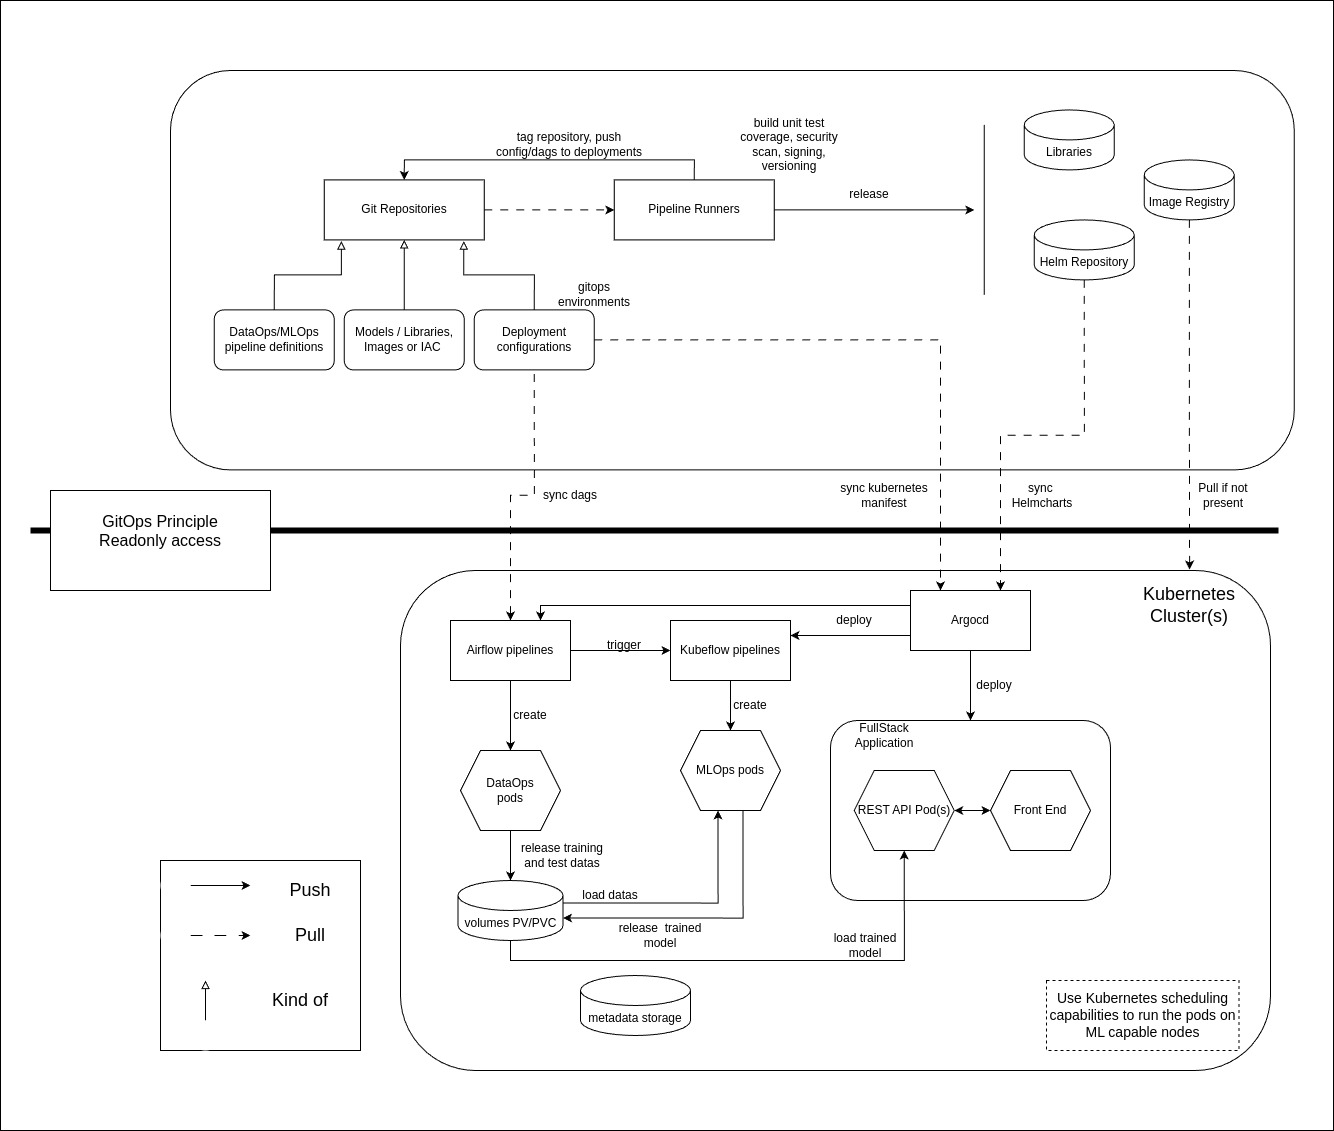
\includegraphics[scale=0.35]{images/project/mthmlops-infra}
    \label{fig:project-infra}
\end{figure}

By using Airflow pipelines as general pipelines to trigger our Kubeflow pipelines, we can easily gain in maturity towards
more automation by combining the DataOps pipelines and MLOps pipelines together when they are mature enough.

This way we enable kubeflow features for our model developers within a more general purpose environment.

By using the git-sync capabilities of Airflow we can synchronise our dags directly with airflow and
even trigger them automatically in a later stage towards automation.

Notably our infrastructure shows the GitOps pull based strategy.
Only the GitHub actions runners do pushes to other git repositories or other
storage like HelmChart repository, images repository or any library repository.
Our Kubernetes environments only pull changes from those repositories, making our infrastructure fully private and easily deployable anywhere.
We will now further describe the component of our workflow.

\subsection{General workflow}\label{subsec:general-development-workflow}
As previously outlined in our state-of-the-art review, the primary triggers for initiating our workflow are either
the emergence of a new development need or the availability of new data.
Beyond the initial phase—during which the project is discussed and defined in collaboration with business stakeholders.
The motivation for further development or model retraining typically arises from the system's monitoring and feedback loops.

Within our GitOps-based MLOps workflow, any change whether in code or configuration must be committed to the appropriate Git repository.
Each push to the repository triggers a DevOps pipeline, which culminate in updating configuration files in a dedicated configuration repository.
This repository is continuously monitored and synchronised by ArgoCD or Airflow, which applies the changes to the cluster and initiates the DataOps pipeline
or integration tests.
Upon successful completion of this stage, the MLOps pipeline is triggered.
If the newly trained model passes validation criteria, it is released to a model repository.
In accordance with GitOps principles, the deployment involves updating configuration files in a separate Git repository,
enabling ArgoCD to automatically deploy the new model version to the production environment thus closing the automation loop
as shown in figure~\ref{fig:general-workflow}.

\begin{figure}[!htbp]
    \centering
    \caption{General Workflow}
    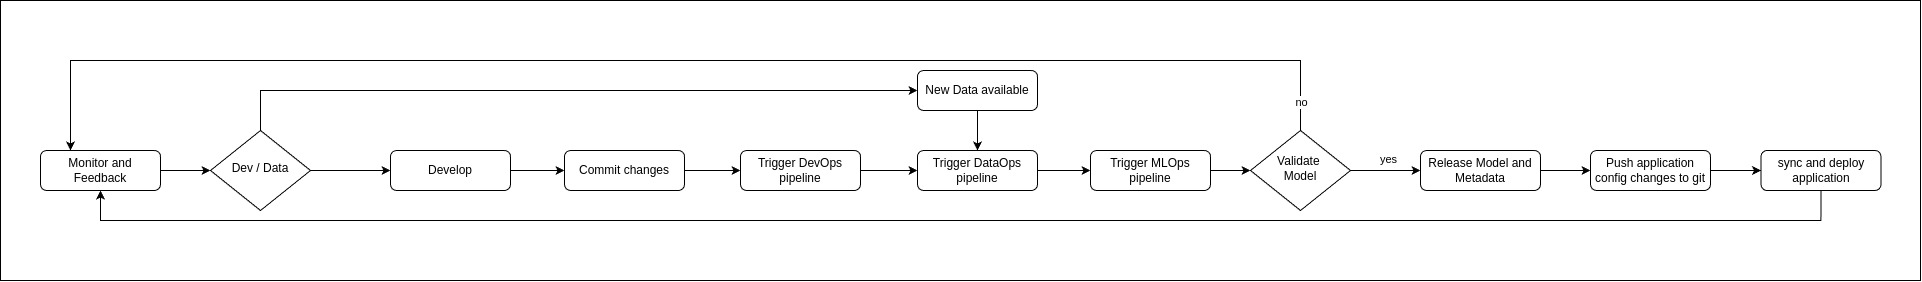
\includegraphics[width=\linewidth]{images/project/general_workflow}
    \label{fig:general-workflow}
\end{figure}

\subsection{Git Repositories}\label{subsec:git-repositories}
As we said, we use Git Repositories for version control and triggering our DevOps pipelines.

Within our infrastructure, we consider 4 types of Git Repositories:

\begin{itemize}
    \item Code Repositories that holds code for models, libraries, docker images and infrastructure as code using Helm.
    \item MLOps and DataOps Pipelines Repositories.
    In our infrastructure those repositories holds the definition of our Airflow DAGs.
    In the first iteration those repositories can also hold images for.
    \item Deployment/Configuration repositories.
    Those repositories are used to hold configuration for the deployed applications and Airflow dags.
    We use ArgoCD GitOps implementation to synchronise changes to those repositories.
    Airflow git/sync feature allows us to synchronise our dags with
    Change in those repositories can be automated by the pipeline runners.
    Depending on your team and organization those repositories can be separated into multiple repositories (per team, per domain, per environment (dev,test,staging,prod))
    For the Dev environment we allow developers to push from their code repositories within those repositories.
    For the production environment we use a pipeline to pull the configuration from the staging environment.
    We called this promote our configuration to a new environment.
    In case of full automation the pulling/promotion can be trigger automatically by ArgoCD sending webhooks on any test results desired.
    \item CI/CD pipelines templates
    In those we define workflows that can be used in any repository to be used by the developers.
    It includes building image workflows, versioning with tags on repositories, pushing new configurations into deployments repositories.
    By defining them in a separate repository it allows us to version them and make it easy for developers to choose a workflow.
    Each workflow is closely tight to the structure of the repository, so we defined one per type of repositories.
\end{itemize}

Following GitOps principle those are the source of truth for all our code and configurations, for the infrastructure, the pipelines, the model and the software development.
We adopt a consistent structure (figure~\ref{fig:sidebyside}) for both our DataOps and MLOps pipeline repositories, incorporating a config.yml file that mirrors the organizational pattern of Helm chart project (values.yaml).
In both cases, an images directory is used to define containerized steps for the pipelines and for deployment configurations within the Helm charts.
This consistency permit to reuse our Devops pipelines templates.

\begin{figure}[h!]
    \centering
    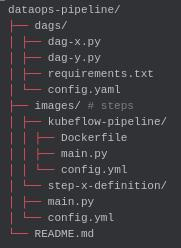
\includegraphics[scale=0.35]{images/project/git-repo-dataops}
    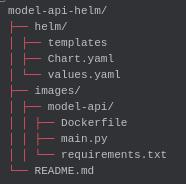
\includegraphics[scale=0.35]{images/project/git-repo-helm}
    \caption{Consistent structure within repositories}
    \label{fig:sidebyside}
\end{figure}


\subsubsection{General Rules for Managing Git Repositories}
We follow the GitHub flow with adaptations to fit our workflow.
However, it can be adjusted as needed.

\begin{itemize}
    \item A Pull Request is required for merging into the \texttt{main} branch, including a pipeline run and team review.
    \item Follow GitHub flow, using \texttt{feature/} and \texttt{hotfix/} branches for development.
    \item Approvals are required for deploying to environment-specific repositories.
    \item The \texttt{main} branch is deployed to the production environment or released into production Docker/Helm repositories.
    \item Other branches are deployed sequentially to all environments, passing tests and approval gates before merging to main.
\end{itemize}

\subsection{GitOps}\label{subsec:gitops2}
With a Helm-based installation pipeline, the runner requires write access to push applications directly to Kubernetes.
By adopting ArgoCD and a GitOps approach, we eliminate this requirement by pulling changes directly from GitHub.
This enables all operations to be managed within GitHub.
However, it necessitates properly configured permissions in GitHub to prevent potential security breaches.

Airflow also integrate a Git/Sync feature that allows us to load and trigger the DAGs within Airflow.

\subsection{DataOps pipelines}\label{subsec:dataops-pipelines2}
DataOps pipelines are defined as Airflow DAGs that will, with the KubernetesExecutor functionality of Airflow,
create pods for every step defined in the pipeline.
They can be connected to an observability stack like OpenSearch or Elasticsearch to analyse and store the data.
Those can be used as Monitoring tools for all our infrastructure too.

\begin{figure}[!htbp]
    \centering
    \caption{Example of a DataOps pipeline define within Airflow}
    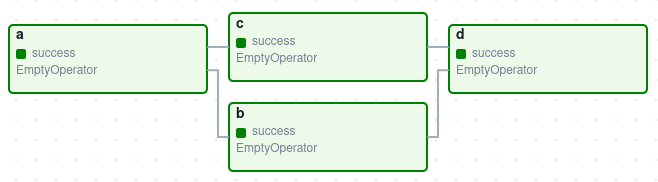
\includegraphics[scale=0.5]{images/project/data-ops-airflow-dag}
    \label{fig:project-data-ops-airflow-dag}
\end{figure}

\subsection{MLOps pipelines}\label{subsec:mlops-pipelines2}
Kubeflow allows us to deploy all the required steps within our MLOps pipeline by creating pods in the required namespace within our Kubernetes cluster.
A lot like Airflow would.
We use Kubeflow to allow our ML engineer to use other features like model and metadata storage.
Other features from the Kubeflow ecosystem could be added at any time if necessary.

\begin{figure}[!htbp]
    \centering
    \caption{Example of a MLOps pipeline define within Airflow}
    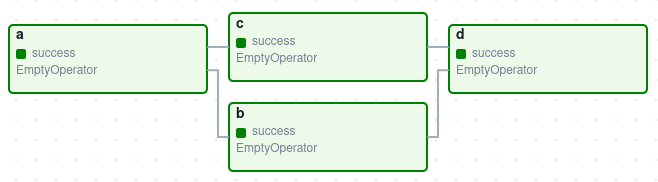
\includegraphics[scale=0.5]{images/project/data-ops-airflow-dag}
    \label{fig:project-ml-ops-airflow-dag}
\end{figure}

\subsection{Storage}\label{subsec:storage}
Here we detail the storage found in our infrastructure (\ref{fig:archi}) and their purpose in our workflow.

\begin{itemize}
    \item Model repository manage by Kubeflow to store our trained, pretrained and untrained models.
    It's an S3 storage that can be mounted as a volume in kubernetes and attached to a running container.
    \item Image repository where we store our container images to be pull by our cluster during deployment.
    \item HelmChart repository to hold and version our infrastructure-as-code templates as packages.
    \item Metadata Database manage by Kubeflow to store model metadata and experiment tracking info.
    \item Git repositories to store code and configuration as already stated.
\end{itemize}

\subsection{Model development}\label{subsec:model-development}
As previously mentioned, we use Helm and Docker to package our model code.
In this section, we'll go into detail about how the model is defined.
The model's Docker image supports three operational modes, each configurable via parameters:
\begin{itemize}
    \item Training mode that loads and trains the untrained model on training data.
    \item A validation mode to load, test and validate the model.
    \item A listen mode define as a REST API server to interface with external frontends or services.
\end{itemize}

To integrate smoothly with our DataOps and MLOps pipelines, we define parameters that specify storage locations.
This ensures that any container image meeting these requirements can be seamlessly used within the pipeline.
Since we use the container layered model, it allows us to take any base image and add a layer that satisfies our pipeline's interface requirements.
While it's convenient to define all stages (training, validation, and listening) within a single image, it may be preferable to split them into two or three separate images.
One downside of the single-image approach is that the model's code is packaged into the same container that's deployed to production.

To deploy our production REST API server to Kubernetes, we created a standard Helm project with template manifests for a Service,
ServiceAccount, Ingress, and Deployment.
In the Helm (values.yaml) configuration file, we specify which trained model version should be loaded, allowing for seamless model hot-swapping when needed.
For more advanced deployment strategies, we can replace the standard Deployment manifest with a Rollout manifest (Custom Resource Definition (CRD) managed by Argo Rollouts).

To use the model within our MLops Kubeflow pipeline, we use our training and validation mode and our data location parameters with Kubeflow Domain specific language container components.
We use the same approach for our DataOps pipelines steps to ensure consistency as we'll demonstrate later in this paper.

% image de argocd api deployment.



\section{Roles within our MLOps workflow}

Each team can be assigned and linked to our type of Git repositories define earlier\ref{subsec:git-repositories}.
All team can receive access to a Deployment/config repository that will be sync to the development environment.
DevOps and Operations teams should be responsible for the production repositories.

As we said earlier deployment repositories are synced to its defined environment but can be isolated using kubernetes namespaces,
and projects within Airflow, Kubeflow\footnote{require Kubeflow installed in multi-user mode} or ArgoCD.
This will ensure any team will deploy to their own namespaces with they predefined resource quotas.

\subsection{DevOps Engineers}
DevOps engineers are responsible for managing CI/CD pipeline templates, repositories, and the underlying runner infrastructure.
They should provide standardized templates for building and releasing Docker images, code libraries, and Helm charts.
Additionally, they should establish a process to synchronize configuration changes from a code repository to a deployment/configuration repository.
\subsection{Data Engineers}
The Data Team is responsible for maintaining at least one DAG repository to define their DataOps pipelines.
For more complex tasks, they should create dedicated code repositories to build custom images used within their DAGs.
\subsection{MLOps Engineers}
MLOps engineers are tasked with defining the overarching workflow and architecture, as demonstrated in this project.
They should oversee and manage relevant tools such as Airflow and Kubeflow, ensuring seamless integration and operation.
\subsection{Model Engineers}
Similar to the Data Team, Model Engineers should maintain at least one DAG repository to define their Kubeflow pipelines and build basic container images.
For more advanced steps, such as model and library development or model training, they should create separate repositories.
These repositories can follow a release workflow and be integrated as dependencies within the pipeline definitions.
\subsection{Software Engineers}
Software Engineers are responsible for developing the application that integrates and utilizes the model,
ensuring it meets functional requirements.
This application is defined as a Helm chart within our workflow, enabling deployment through ArgoCD.
For advanced deployment strategies, ArgoCD Rollouts can be utilized to ensure more refined and controlled release processes.
The trained model version is integrated into a REST API component, which is part of the application.

\subsection{Example of minimal list of git repositories per roles/teams within an Organisation}

\begin{minted}{markdown}
Organisation
    -> DevOps Project
        -> CI/CD pipelines templates
    -> DataOps Project
        -> Airflow DAG definition with image for simple steps
        -> dataops-step-x
        -> dataops-step-y
    -> ML Project
        -> model code repository
        -> DAG/kubeflow pipeline repository
        -> mlops-pipeline-step-1
    -> ML Ops project
        -> Airflow/Kubeflow configuration
        -> infrastructure definition
    -> Operations
        -> production environment repositories subject to different rules.
\end{minted}

\section{Workflows}\label{sec:workflow}

\subsection{DevOps CI/CD pipelines}\label{subsec:ci/cd-pipelines-and-development-workflow}
As we explained while describing the infrastructure, part of our global workflow can be implemented within pipelines runners definition.
We used GitHub action and the GitHub flow to harmonise the workflow within our different type of git repositories.
GitHub allows us to define template in a single repository that can be then versioned and used in other repositories while hiding the complexity of the defined pipelines.
We also followed the GitHub flow which involve one main branch and features or hotfix branch to favor small and fast release.
As stated before other strategies can be used with an adapted development workflow.

\begin{figure}[!htbp]
    \centering
    \caption{Implementation of the GitHub Flow CI/CD workflow}
    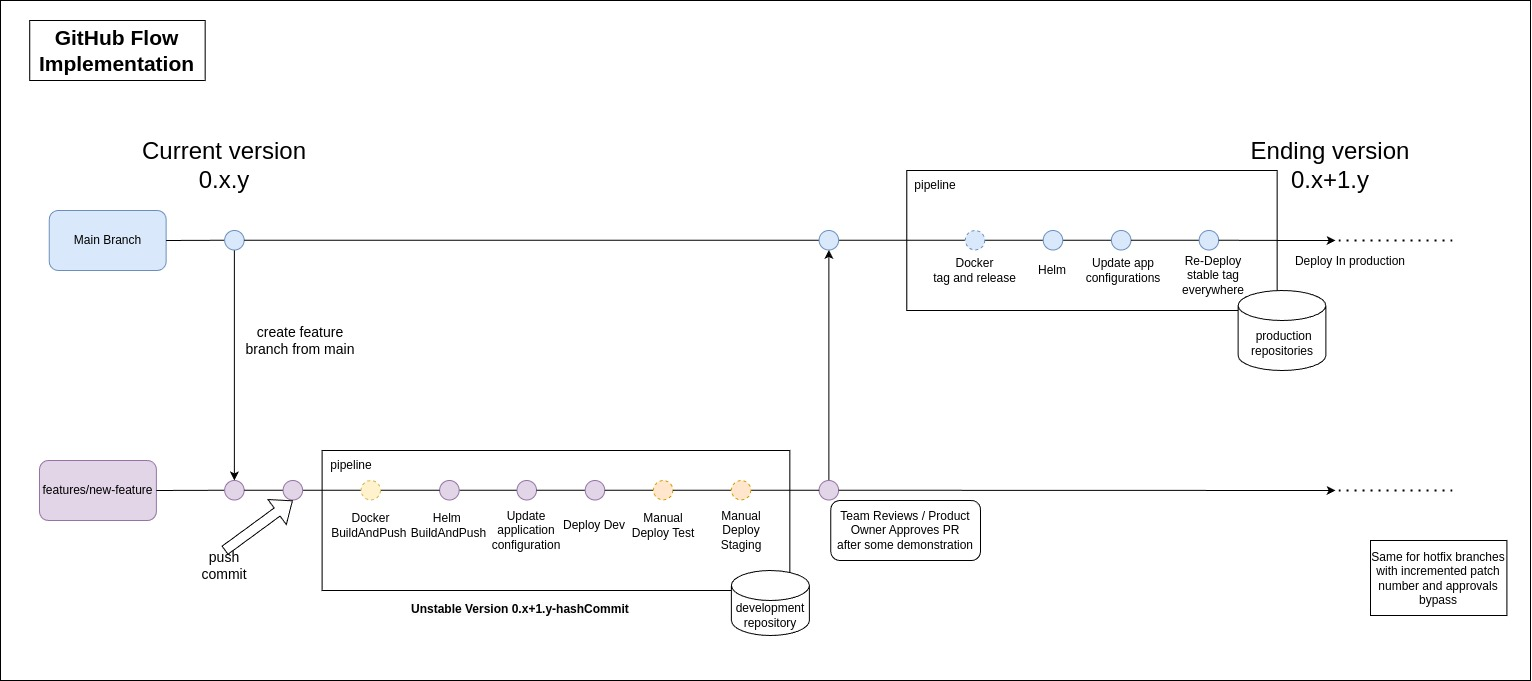
\includegraphics[scale=0.3]{images/project/cicd-workflow-p1}
    \label{fig:icd-workflow-p1}
\end{figure}

There are our development pipelines for any git repositories except for the deployment repository that are only targets.
Artifact that are not deployed but released to a directory follows the same path but are deployed as dependencies within other projects.
Airflow DAGS follows the same development workflow and are release into our previously defined git deployment repositories.

\begin{figure}[!htbp]
    \centering
    \caption{Development Team Contribution activity}
    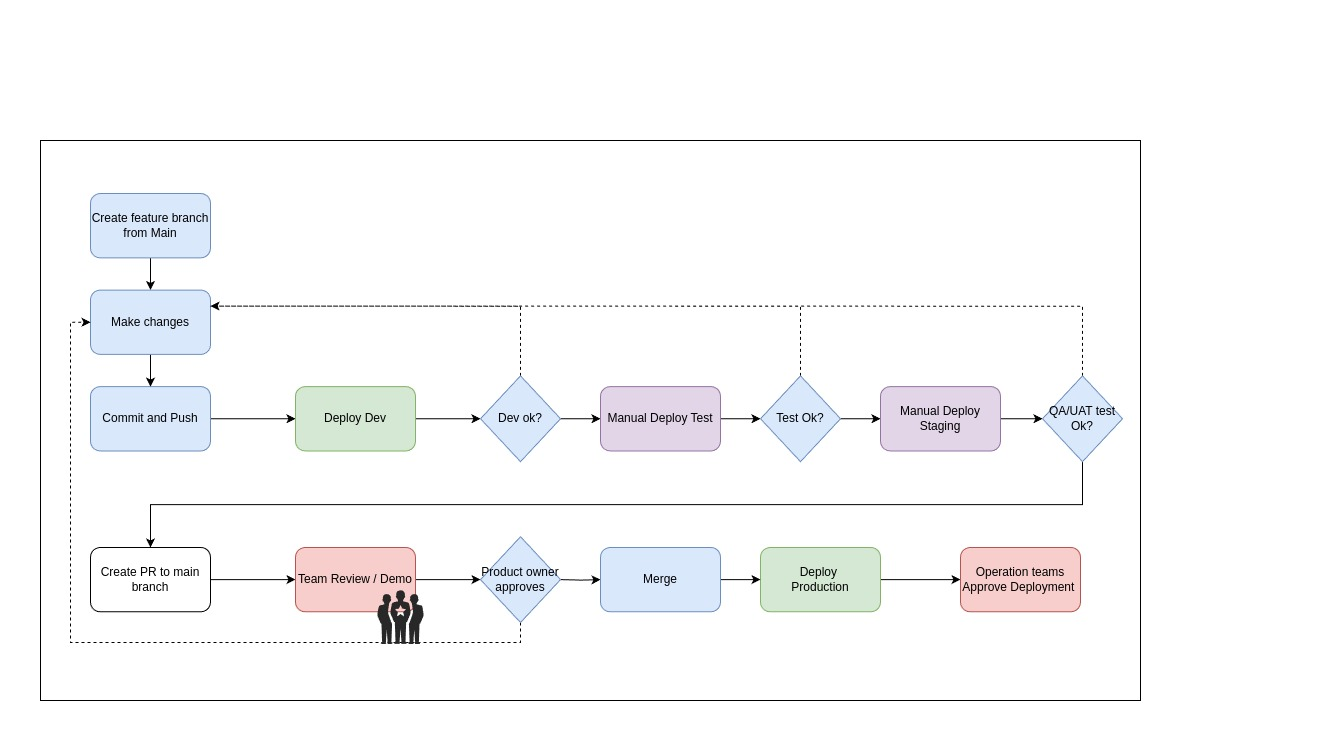
\includegraphics[scale=0.3]{images/project/cicd-workflow-p2}
    \label{fig:cd-workflow-p2}
\end{figure}


\subsection{DataOps pipelines}\label{subsec:dataops-pipelines}
Inspired by our research in the literature we create a sample DataOps pipeline that can be implemented with specific
operations.

\begin{figure}[!htbp]
    \centering
    \caption{DataOps sample workflow}
    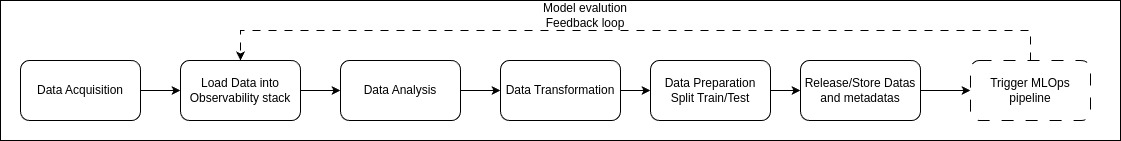
\includegraphics[scale=0.3]{images/project/dataops-workflow}
    \label{fig:dataops-workflow}
\end{figure}

It's defined in our project as an Airflow DAG and can be triggered manually in early stage of the project or
automatically when the project has enough maturity.

\subsection{MLOps pipelines}\label{subsec:mlops-pipelines}
Our MLOps pipelines are developed as Kubeflow pipelines with the possibility to trigger them from an airflow DAG
even in the early stage of the project in ensure the possibility to combined it with the DataOps pipeline to advance towards AutoML.


\section{Future Work}\label{sec:future-work}
Our project is currently a prototype that can be used in development and testing environments.
Future project should implement this in production.
The current implementation still lack some of the consideration explained before and a more mature DevOps infrastructure.
We focused on the MLOps part and workflow but .

Add a vault secret manager for secret management \url{https://argo-cd.readthedocs.io/en/stable/operator-manual/secret-management/}.

We used the ArgoCD the app-of-apps pattern in our implementation but to offer more self-service to development teams it could be interesting to use application sets

At the moment we think it's usefully to use 3 different pipeline orchestrator, but it's probable that in the future we could use only one as
GitHub now propose a Model registry, Kubeflow is extending its Data management and Airflow is also going towards more MLOPs integration.

\url{https://argo-cd.readthedocs.io/en/stable/operator-manual/applicationset/Use-Cases/#use-case-self-service-of-argo-cd-applications-on-multitenant-clusters}.


\section{Conclusion}\label{sec:conclusion}
Airflow pipelines and Kubeflow pipelines to easily integrate DataOps and MLOps pipelines together to reach more automation as the project gains maturity.
By using the same GitOps workflow for our DataOps and MLOps pipelines that for our HelmCharts to deploy our infrastructure and applications,
we successfully

We